\chapter{Experimental Evaluation}
\label{sec:experiment}


In this chapter, we evaluate the performance of our proposed
\bptree and show the experimental results. An extensive performance study is conducted to show the
efficiency and effectiveness of the \bptree with various types of
queries and updates. Since we have not got any PCM prototype in hand, we need to setup an environment
to simulate the PCM characteristics first. Then we did our experiments in the simulated environment.
Our results show \bptree outperforms the traditional \bplustree on the insertion and deletion performance,
while holding a similar search performance at the same time.

\section{Experimental Setup}

In this section, we are going to present our experimental setup. We talk about the
experimental platform first and we will present the details of our simulation platform.
After that we will propose our data set, workloads and the different algorithms we are going to compare with.

\subsection{Experimental platform}

We integrate our proposed
\bptree in PostgreSQL and extend the buffer management module to
support the PCM model. We follow the specifications of the PCM
model in~\cite{chen2011rethinking} and we also talked about this in Chapter~\ref{sec:technology}.
Three metrics are used in our
experiments to measure the performance the \bptree, namely the
number of writes, energy consumption and CPU cycles.
%
Each time when we write a new cache line into the PCM, we compute the number
of modified bits and bytes by comparing it with the previous one.
In our experiments, the number of writes is computed as the
number of modified bytes, while the energy consumption is estimated
by the number of modified bits. We compute the CPU cost by
combining the CPU cycles of our \bptree in both PCM and DRAM.
%For the CPU cycles, we  the CPU cost of the \bplustree in DRAM buffer of our \bptree.

The experiments were conducted in CentOS release 5.6 with g++
4.1.2. Our system is powered with a 16-core Intel Xeon E5620
2.4GHz CPU and 64GB main memory. Based on the benchmark used
in~\cite{chen2011rethinking,qureshi2009scalable,bedeschi2008multi},
we set the parameters as follows: the read latency of a PCM cache
line is 288 cycles; the write latency of PCM is 281 cycles for
every 4 bytes; the read latency of a DRAM cache line is 115 cycles
and the write latency of DRAM is 7 cycles for every 4 bytes. In
PCM, the energy consumption is estimated as: the read energy per
bit is 2pJ and the write energy per bit is 16pJ. In
Table~\ref{tab:parameter}, we list the other parameters used in
our experiments and their value ranges.


\begin{table}\vspace*{-1em}
\centering
\caption{Parameters and their value ranges}
\label{tab:parameter}
\hspace*{-1em}
\begin{tabular}{|c|c|}
 \hline
 \bf Parameter & \bf Value Ranges \\
 \hline
 \hline Size of DRAM buffer&5\% of the size of the PCM used\\
 \hline Size of cache line&64B\\
 \hline Size of the \bplustree node& 256B (4 cache lines)\\
 \hline Size of the \bptree node&256B, 512B, 1024B \\
    &(4, 8, 16 cache lines)\\
 \hline K&1, 2, 4\\
 \hline Number of keys in &5 millions\\
    the data set & \\ \hline
\end{tabular}
\end{table}

%\vspace{.5em}

\subsection{Data sets and workloads}

Two synthetic datasets
are used in our experiments. One is generated to follow the
uniform distribution, while the other one follows the skewed
distribution. We generate 5 millions keys in each dataset. In our
experiments, the node size of the DRAM \bplustree is 256B, which
is equivalent to 4 cache lines; whereas the node size of all tree
structures on the PCM varies from 256B, 512B to 1024B. In our
\bptree, each index entry contains a 4-Byte key and a 4-Byte
pointer. The size of the DRAM buffer used is approximately 5\% of
the size of the PCM. We generate various workloads (i.e.,
insertions, updates and searches) to study the performance of our
approach. Specifically, an update is processed as a deletion
operation followed by an insertion operation, and the search
queries are composed of both the point queries and range queries.
Based on our experimental results, we find that the performance on
uniform dataset is similar to that on skewed dataset. Therefore,
we only report the results on skewed dataset.

\vspace{.5em}

\subsection{Algorithms compared}

We compare four different
indexing structures including our \bptree, the traditional
\bplustree, the proposed Unsorted Leaf tree
in~\cite{chen2011rethinking} and our \bptree with sorted leaf
nodes on the basis of the following measures, the number of writes during the insertions, the energy consumption,
the CPU cycles (including the small \bplustree in the DRAM for \bptree) during the insertions and searches, and the leaf nodes utilization.

As the \bptree is a composite structure including the main \bptree
on PCM and the small buffer \bplustree on DRAM, we need to
determine how to compute each performance metric first. In the
performance evaluation, we only consider the PCM cost while
calculating the number of writes and the energy consumption. As
for the CPU cost, the CPU cycles occupied for manipulating the
DRAM \bplustree are recorded, which can represent a more accurate
processing time. All the indexes are tuned and only the best results are reported.

In all figures presented in this section, ``BP-tree'' represents
our \bptree; ``B-tree'' represents the traditional \bplustree;
``Unsorted'' represents the proposed unsorted leaf tree
in~\cite{chen2011rethinking}; and ``BP-minus'' represents \bptree
with sorted leaf nodes. The x-axis represents the node size of the
corresponding tree, e.g., x-coordinates 4 indicates that the node
size of the corresponding tree is 4 cache lines.

\section{Results and Analysis}

We did various of experiments and in this chapter, we will show the results including insertion, update, search and node utilization.
At last, we also did some more experiments to show that our \bptree indexing can work well under different data distributions.

\subsection{Insertion}
We first evaluate the insertion performance of \bptree. We insert
all the keys in the dataset back-to-back using the different indexing algorithms. 
%and the measures include number of writes, energy consumption and CPU cycles.
Moreover, for each data set, we build the tree using three different node sizes, that is, 4, 8, 16 cache lines, respectively.

\begin{figure*}[!t]
\centering

\subfigure[Writes]{
    \includegraphics[scale = 0.55] {figs/zipf_result11.eps}
    \label{fig:exp:insertion:subfig12}
} \subfigure[Energy]{
    \includegraphics[scale = 0.55] {figs/zipf_result12.eps}
    \label{fig:exp:insertion:subfig22}
} \subfigure[Cycles]{
    \includegraphics[scale = 0.55] {figs/zipf_result13.eps}
    \label{fig:exp:insertion:subfig32}
}

\caption{Insertion performance} \label{fig:exp:insertion}
\end{figure*}

In Figure~\ref{fig:exp:insertion}, we compare the insertion
performance of  four tree indexing schemes. The three subfigures
correspond to our three metrics respectively. In each subfigure,
we present the performance of the four tree structures with three
different node sizes. The scale of y-axis in Figure~\ref{fig:exp:insertion}(a)
and (b) are both in millions. We get two interesting observations from the results.

First, our \bptree achieves the best performance on all the three
metrics and the performance gap increases as the node size becomes
larger. The reason is that for large node sizes, our predictive model
can estimate the splits more accurately, which can significantly
reduce the number of writes by avoiding online splitting. On the
other hand, Unsorted  outperforms \bplustree and BP-minus. This is
because most  writes will appear in leaf nodes and Unsorted can
reduce the number of writes on leaf nodes. Our \bptree outperforms
the Unsorted scheme, as it splits the nodes in advance, which can
reduce the numbers of future splits. \bptree incurs  about 5\%,
22\%, 37\%  less PCM writes than the Unsorted scheme on the three
different node sizes respectively. For energy consumption, the
result is very similar to that of the writes. For CPU cycles, the
gap becomes slightly smaller because \bptree incurs extra CPU
costs on the small \bplustree in the DRAM buffer. However, \bptree
still performs better than the Unsorted tree by a factor of 18\%
when the node size is 16 cache lines.

Second, we compare the performance of the two tree indexes with
sorted leaf nodes, namely BP-minus and \bplustree. BP-minus
outperforms \bplustree in all metrics. BP-minus reduces about
25\%, 33\%, 42\% of numbers of PCM writes compared to the
\bplustree. Similar trend is observed for the energy
consumption. This means that our \bptree outperforms the traditional 
\bplustree even if we do not want to make the keys on each node unsorted.
 For CPU cycles, the gap is not that significant
because of the extra cost on the small \bplustree in the DRAM
buffer. Despite this, BP-minus still reduces 14\%, 22\%, 35\% cost
of that of \bplustree.

\subsection{Update}

In this section, we evaluate the update performance of \bptree. We
first insert all the keys back-to-back as the previous insertion
experiment and then we generate and run 100k update queries
randomly. The update query consists of two keys, $oldKey$ and
$newKey$. We first search the $oldKey$. If we find it, we delete
it and insert the $newKey$. Otherwise, we will ignore the
insertion request. In Figure~\ref{fig:exp:update}, we compare the
average update performance of our \bptree and the other three tree
structures. The result is very close to that of the insertion
performance.

Our \bptree still achieves the best performance on all the three
measures. The main reason is that our \bptree can predict future
insertions and can pre-allocate space to reduce the number of
writes. Compared to Unsorted, our \bptree reduces 24\% of the
writes, 26\% of the energy and 19\% of the CPU cycles, when the
node size is 16 cache lines. If the node size is small, the gap
decreases but our \bptree still outperforms Unsorted.

Compared to the traditional \bplustree, the performance of
BP-minus is better. It reduces 14\% of the writes, 22\% of the
energy and 7\% of the CPU cycles and the gap increases as the node
size becomes larger. It shows the similar trends for all of the three measures.

\begin{figure*}[!t]
\centering

\subfigure[Writes]{
    \includegraphics[scale = 0.55] {figs/zipf_result81.eps}
    \label{fig:exp:update:subfig12}
} \subfigure[Energy]{
    \includegraphics[scale = 0.55] {figs/zipf_result82.eps}
    \label{fig:exp:update:subfig22}
} \subfigure[Cycles]{
    \includegraphics[scale = 0.55] {figs/zipf_result83.eps}
    \label{fig:exp:update:subfig32}
}

\caption{Update performance} \label{fig:exp:update}
\end{figure*}

\subsection{Search}

\begin{figure}[!t]
\centering

\subfigure[Point Query]{ \hspace*{-2em}\includegraphics[scale =
0.55] {figs/zipf_result4.eps}
    \label{fig:exp:search:subfig12}
} \subfigure[Range Query]{ \hspace*{-2em}\includegraphics[scale =
0.55] {figs/zipf_result6.eps}
    \label{fig:exp:search:subfig22}
}

\caption{Search performance} \label{fig:exp:search}
\end{figure}

The philosophy of \bptree is two-fold: 1) \bptree is designed to
reduce the number of writes on PCM, and 2) \bptree should be
efficient for query processing as well. In this section, we
evaluate the search performance of \bptree. The experiments
include point queries and range queries. We experiment on both the
uniform and skewed datasets. We first insert all  keys into the
index. Then for both point query and range query, we randomly
generate 50k queries and  calculate the CPU cycles during the
processing.


In Figure~\ref{fig:exp:search}, we compare the search performance
of the four tree indexes. The left subfigure is for point query
and the right one is for range query. The y-axis represents the total
CPU cycles to run these search queries. For point query, the
performance of \bptree is better than Unsorted. This is because
when we process the search query, we simply scan the node and once
we find the key, we will return the associated data.
%%%%%cannot understand
If the \bptree has more leaf nodes than Unsorted, some keys
located in the right part of some nodes in Unsorted may be in the
left part of some nodes in \bptree and thus more cache line reads
are needed.
%%%%%%
The performance of BP-minus is better than that of Unsorted, which
is expected since each search in Unsorted should read all the keys
in the leaf node.



For range query, we can find that when the node size is 4 cache
lines, the performance of our \bptree and BP-minus is worse than
that of the \bplustree and Unsorted. The reason is that when the
node size is small, the tree will be more sensitive to the split
strategy and generate more leaf nodes which could affect the range
search performance. When the node size is larger, all the four
tree indexes show a similar performance. This result is very important
which means that the indexing tree is in a good shape and it did not
split too ``early'' and make the tree too sparse. 



\subsection{Node Utilization}

In this experiment, we compare the leaf node utilization of the
\bptree and the traditional \bplustree. The experiments are same
as the insertion performance experiment and we build the two trees
based on the same data set and calculate the leaf nodes
utilization periodically during the insertion. The scale of the x-axis is 
0.5 million which means that 8 represents 4 millions keys inserted. The suffixes -4,
-8, -16  in the figure indicate different node sizes. 

As we can see in the figure, the leaf node utilization of the \bplustree is
stable, around 70\% which is close to our assumption in
Section~\ref{sec:cost}. When the node size of the \bptree is 4
cache lines which is the same as that of the \bplustree, the
utilization is similar to that of the \bplustree at first and then
decreases as early splits happen and then it increases as the
evaluation metrics described in Section~\ref{sec:cost} starts to
work. When the node size is 8 cache lines, the utilization is
smaller than that of the \bplustree at first because of the enlargement of
the node size and then it starts to increase. The result for the
node size of 16 cache lines is similar. The stable utilization of
all the three different \bptree indexes are all slightly smaller
than that of the traditional \bplustree, but according to the
previous range search experiment, the influence of the utilization
gap on the range search performance is not obvious and it is affordable.

\begin{figure}[!t]
\centering
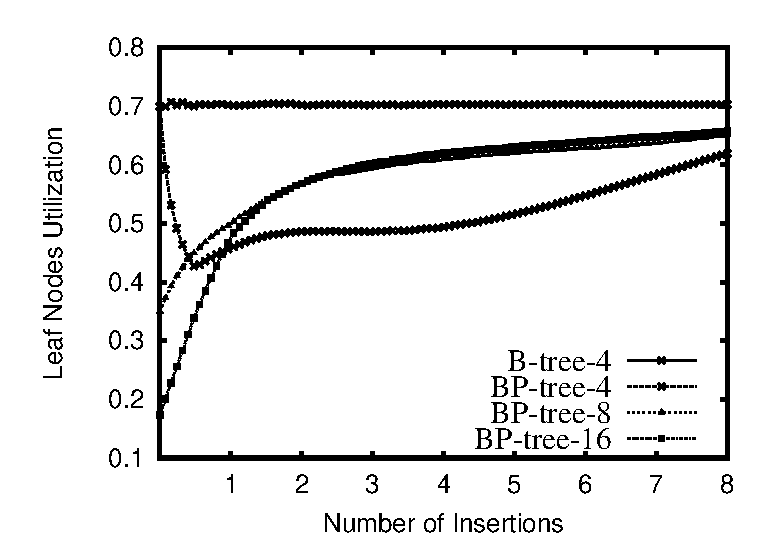
\includegraphics[scale = 0.65] {figs/zipf_result5.eps}

\caption{Leaf nodes utilization} \label{fig:exp:utilization}
\end{figure}

\subsection{Sensitivity to Data Distribution Changes}
In this section, we evaluate the sensitivity of our predictive
model to data distribution changes in order to show that our \bptree is stable
with the dataset of different data distributions. We change the dataset as
follows. The size of the dataset is 5 millions and the dataset follows
a skewed (Zipf) distribution. However, we gradually change the Zipf factors and
add a random offset every one million keys generated,
resulting in a change of the data distribution. We did
the insertion, update, search experiments as in previous sections.
In Figure~\ref{fig:exp:sensitivity}, we show comparisons of the
CPU cycles of all the four tree indexes with respect to different
operations.


From the figure, we can observe that the relative performance of
insertion, update and point search is very similar to that of the
previous experiments. For the leaf node utilization, when the node
size is 4 cache lines, the trend of the first half is similar to
that of the previous result, but the utilization decreases slightly
as the second half starts and increases again at last. The
reason of the decrease is that changes of data distribution caused
a wrong prediction from the predictive model and further caused
some improper splits. After that the predictive model adjusts its
prediction via the evaluation metrics and makes the structure
normal again which means that our evaluating scheme works fine 
and it can help the predictive model to modify the splitting strategy. 


We can also observe from Figure~\ref{fig:exp:sensitivity}(e) that
the stable utilization value is a bit smaller than that of the
previous experiments, which may have also caused the range search
performance to degrade slightly as shown in
Figure~\ref{fig:exp:sensitivity}(d). To summarize, the major
performance of the \bptree verified in the previous experiments
still holds when the data distribution changes which shows \bptree to be stable.

\begin{figure*}[!t]
\centering
\subfigure[Insertion]{
    \hspace*{-1.5em}\includegraphics[scale = 0.55] {figs/zipf_result921.eps}
    \label{fig:exp:sensitivity:subfig1}
} \subfigure[Update]{
    \hspace*{-1.5em}\includegraphics[scale = 0.55] {figs/zipf_result924.eps}
    \label{fig:exp:sensitivity:subfig2}
} \subfigure[Point Search]{
    \hspace*{-1.5em}\includegraphics[scale = 0.55] {figs/zipf_result922.eps}
    \label{fig:exp:sensitivity:subfig3}
} \subfigure[Range Search]{
    \hspace*{-1.5em}\includegraphics[scale = 0.55] {figs/zipf_result923.eps}
    \label{fig:exp:sensitivity:subfig4}
} \subfigure[Leaf Node Utilization]{
    \hspace*{-1.5em}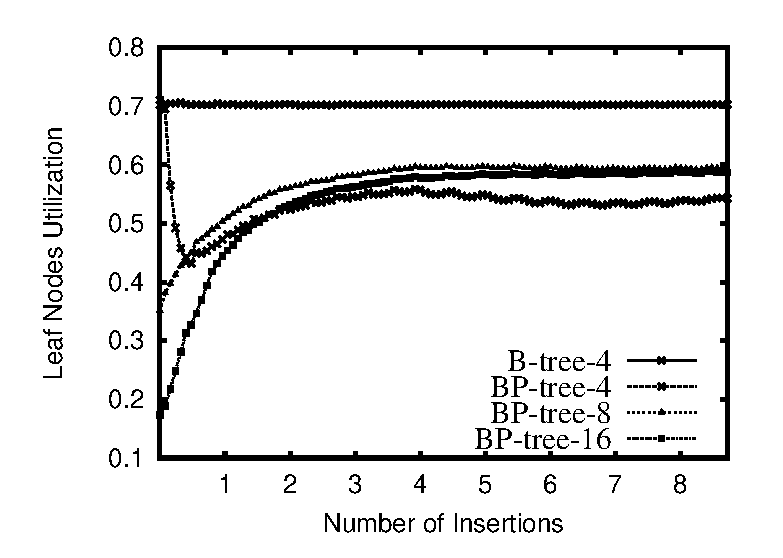
\includegraphics[scale = 0.55] {figs/zipf_result925.eps}
    \label{fig:exp:sensitivity:subfig5}
} \caption{Sensitivity to Data Distribution Changes}
\label{fig:exp:sensitivity}
\end{figure*}

\section{Summary}

In this chapter, we did an extensive experiments evaluation of our \bptree. We build our experimental
platform to simulate the PCM environment and compare it with some of the other write-optimized indexing
technique and the traditional normal \bplustree. We did the experiments based on both the uniform
dataset and skewed dataset. We observed that for both data distribution, our \bptree can work well.
The experimental results show that the \bptree significantly reduces
the number of writes for both the insertions and updates while having a good search performance at the same time,
therefore making it write and energy efficient and suitable for a PCM-like
hardware environment. The sensitivity experiments show that \bptree is a stable indexing technique and 
it works fine for different datasets. 


\newpage
